\lstinputlisting[firstline=33, lastline=36]{Prozeduren.rkt}
Eine Signatur pr\"uft, ob ein Name an einen Wert einer angegebenen Sorte (Typ) gebunden wird. Signaturverletzungen werden protokolliert.\\
\lstinline!(: <id> <signatur>)!\\
Bereits eingebaute Sinaturen\\
\begin{tabular}{rc|r}
natural&$\mathbb{N}$& boolean\\
integer&$\mathbb{Z}$& string\\
rational&$\mathbb{Q}$& image\\
real&$\mathbb{R}$&$\ldots$\\
number&$\mathbb{C}$
\end{tabular}\\
\lstinline!(: ...)! ist eine Spezialform und hat keinen Wert, aber einen Effekt: Signaturprüfung\\
\uline{Prozedur Signatur} spezifizieren sowohl Signaturen f\"ur die Parameter $\text{P}_1,\text{P}_2,\ldots\text{P}_n$ als auch den Ergebniswert der Prozedur,\\
\lstinline[literate=]!(: <Signatur P1> ... <Signatur Pn> -> <Signatur Ergebnis>)!\\
Prozedur Signaturen werden \emph{bei jeder Anwendung} einer Prozedur auf Verletzung gepr\"uft. \emph{Testf\"alle} dokumentieren das erwartete Ergebnis einer Prozedur f\"ur ausgew\"ahlte Argumente:
\begin{center}
\lstinline[literate=]!(check-expect <e1> <e2>)!\end{center}
Werte Ausdruck \auf $\text{e}_1$\zu \ aus und teste, ob der erhaltene Wert der Erwartung \auf $\text{e}_2$\zu \ entspricht (= der Wert von \auf $\text{e}_2$\zu) \
Einer Prozedur sollte Testf\"alle direkt vorangestellt werden.\\
Spezialform: kein Wert, sondern Effekt: Testverletzung protokollieren\\
\emph{Konstruktionsanleitung f\"ur Prozeduren:}
\begin{enumerate}
\item[(1)]Kurzbeschreibung (ein- bis zweizeiliger Kommentar mit Bezug auf Parametername)
\item[(2)]Signaturen
\item[(3)]Testf\"alle
\item[(4)]Prozedurrumpf
\end{enumerate}
\emph{Top-Down-Entwurf} (Programmieren durch ``Wunschdenken``)\\
Beispiel: Zeichne Ziffernblatt (Stunden- und Minutenzeiger) zu Uhrzeit h:m auf einer analogen 24h-Uhr\\
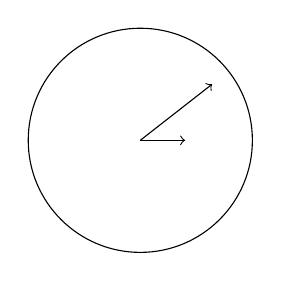
\begin{tikzpicture}
    \begin{axis}[
    legend style={draw none},
    axis equal,ymin = -2,xmin = -2,ymax = 2,
    xmax = 2,xtick ={},
    hide axis,
    xticklabels={},
    ytick ={},
    yticklabels={},
    extra x ticks={0},
    extra x tick label={},
    extra y ticks={0},
    extra y tick labels={},
    disabledatascaling,
    extra tick style = {grid = major}]
    \draw (axis cs:0,0) circle[radius=1];
    \draw[->](axis cs:0,0)--(axis cs:0.64,0.5);
    \draw[->](axis cs:0,0)--(axis cs:0.4,0);
    \end{axis}   
  \end{tikzpicture}\\
  Minutenzeiger legt $\frac{360^{\circ}}{60}$ Grad pro Minute zur\"uck (also $\frac{360}{60} \cdot m$)\\
  Studentenzeiger legt $\frac{360}{12}$ pro Stunde zur\"uck
 ($\frac{360}{12} \cdot h +\frac{360}{12} \cdot \frac{m}{60}$)
 \rackett{Bilderzusammenstellung am Beispiel einer Uhr}{Bauen der Uhr durch Top Down Entwurf}{Prozeduren}{44}{87}
